\begin{filecontents*}{\jobname.bib}
@article{hossen2023bert,
  author  = {Kazi Mojammel Hossen and Mohammed Nasir Uddin and Minhazul Arefin and Md Ashraf Uddin},
  title   = {{BERT} Model-based Natural Language to {NoSQL} Query Conversion using Deep Learning Approach},
  journal = {International Journal of Advanced Computer Science and Applications},
  volume  = {14},
  number  = {2},
  pages   = {810--821},
  year    = {2023}
}
@article{tend2025benchmark,
  author  = {Jinwei Lu and Jiawei Lu and Chen Zhang and Zhiqian Qin and Haodi Zhang and Yuanfeng Song and Raymond Chi-Wing Wong},
  title   = {Bridging the Gap: Enabling Natural Language Queries for {NoSQL} Databases through {Text-to-NoSQL} Translation},
  journal = {arXiv preprint arXiv:2502.11201},
  year    = {2025},
  note    = {version 3}
}
@inproceedings{spider2018,
  author    = {Tao Yu and Rui Zhang and Kai Yang and Michihiro Yasunaga and Dongxu Wang and Zifan Li and James Ma and Irene Li and Qingning Yao and Shanelle Roman and Zilin Zhang and Dragomir Radev},
  title     = {{Spider}: A Large-Scale Human-Labeled Dataset for Complex and Cross-Domain Semantic Parsing and {Text-to-SQL} Task},
  booktitle = {Proceedings of the 2018 Conference on Empirical Methods in Natural Language Processing (EMNLP)},
  pages     = {3911--3921},
  year      = {2018}
}
@inproceedings{bird2023,
  author    = {Jinyang Li and Binyuan Hui and Ge Qu and Jiaxi Yang and Binhua Li and Bowen Li and Bailin Wang and Bowen Qin and Ruiying Geng and Nan Huo and Xuanhe Zhou and Chenhao Ma and Guoliang Li and Kevin C. C. Chang and Fei Huang and Reynold Cheng and Yongbin Li},
  title     = {Can {LLM} Already Serve as a Database Interface? {A} {BIg} Bench for Large-Scale Database Grounded {Text-to-SQLs}},
  booktitle = {Advances in Neural Information Processing Systems},
  volume    = {36},
  pages     = {42330--42357},
  year      = {2023}
}
@inproceedings{dinsql2023,
  author    = {Mohammadreza Pourreza and Davood Rafiei},
  title     = {{DIN-SQL}: Decomposed In-Context Learning of {Text-to-SQL} with Self-Correction},
  booktitle = {Advances in Neural Information Processing Systems},
  volume    = {36},
  pages     = {36339--36348},
  year      = {2023}
}
@article{dailsql2023,
  author  = {Dawei Gao and Haibin Wang and Yaliang Li and Xiuyu Sun and Yichen Qian and Bolin Ding and Jingren Zhou},
  title   = {{Text-to-SQL} Empowered by Large Language Models: A Benchmark Evaluation},
  journal = {Proceedings of the VLDB Endowment},
  volume  = {17},
  number  = {5},
  pages   = {1132--1145},
  year    = {2024}
}
@article{docspider2025,
  author  = {A. G. {\"O}zer and R. F. Cekinel and I. H. Toroslu and P. Karagoz},
  title   = {{DocSpider}: A Dataset of Cross-Domain Natural Language Querying for {MongoDB}},
  journal = {Natural Language Processing},
  volume  = {31},
  number  = {6},
  pages   = {1367--1398},
  year    = {2025}
}
@inproceedings{multitend2025,
  author    = {Zhiqian Qin and Yuanfeng Song and Jinwei Lu and Yuanwei Song and Shuaimin Li and Chen Jason Zhang},
  title     = {{MultiTEND}: A Multilingual Benchmark for Natural Language to {NoSQL} Query Translation},
  booktitle = {Findings of the Association for Computational Linguistics: ACL 2025},
  pages     = {24632--24657},
  year      = {2025}
}
@inproceedings{sm3text2024,
  author    = {Sithursan Sivasubramaniam and Cedric Osei-Akoto and Yi Zhang and Kurt Stockinger and Jonathan F{\"u}rst},
  title     = {{SM3-Text-to-Query}: Synthetic Multi-Model Medical Text-to-Query Benchmark},
  booktitle = {Advances in Neural Information Processing Systems},
  volume    = {37},
  pages     = {88627--88663},
  year      = {2024}
}
@article{quamar2022nli,
  author  = {Abdul Quamar and Vasilis Efthymiou and Chuan Lei and Fatma {\"O}zcan},
  title   = {Natural Language Interfaces to Data},
  journal = {Foundations and Trends in Databases},
  volume  = {11},
  number  = {4},
  pages   = {319--414},
  year    = {2022}
}
@inproceedings{ozcan2020nli,
  author    = {Fatma {\"O}zcan and Abdul Quamar and Jaydeep Sen and Chuan Lei and Vasilis Efthymiou},
  title     = {State of the Art and Open Challenges in Natural Language Interfaces to Data},
  booktitle = {Proceedings of the ACM SIGMOD International Conference on Management of Data},
  pages     = {2629--2636},
  year      = {2020}
}
@inproceedings{blank2019nosql,
  author    = {Sebastian Blank and Florian Wilhelm and Hans-Peter Zorn and Achim Rettinger},
  title     = {Querying {NoSQL} with Deep Learning to Answer Natural Language Questions},
  booktitle = {Proceedings of the AAAI Conference on Artificial Intelligence},
  volume    = {33},
  number    = {1},
  pages     = {9416--9421},
  year      = {2019}
}
@inproceedings{fast2018iris,
  author    = {Ethan Fast and Binbin Chen and Julia Mendelsohn and Jonathan Bassen and Michael S. Bernstein},
  title     = {Iris: A Conversational Agent for Complex Tasks},
  booktitle = {Proceedings of the 2018 CHI Conference on Human Factors in Computing Systems},
  pages     = {1--12},
  year      = {2018}
}
@manual{mongodb2024manual,
  author       = {{MongoDB, Inc.}},
  title        = {Aggregation Pipeline, {MongoDB} Manual},
  howpublished = {\url{https://www.mongodb.com/docs/manual/core/aggregation-pipeline/}},
  note         = {Accessed: Oct. 2026},
  year         = {2024}
}
@inproceedings{aliannejadi2019asking,
  author    = {Mohammad Aliannejadi and Hamed Zamani and Fabio Crestani and W. Bruce Croft},
  title     = {Asking Clarifying Questions in Open-Domain Information-Seeking Conversations},
  booktitle = {Proceedings of the 42nd International ACM SIGIR Conference on Research and Development in Information Retrieval (SIGIR)},
  pages     = {475--484},
  year      = {2019}
}
@inproceedings{zamani2020generating,
  author    = {Hamed Zamani and Susan T. Dumais and Nick Craswell and Paul N. Bennett and Gord Lueck},
  title     = {Generating Clarifying Questions for Information Retrieval},
  booktitle = {Proceedings of the Web Conference (WWW)},
  pages     = {418--428},
  year      = {2020}
}
@inproceedings{min2020ambigqa,
  author    = {Sewon Min and Julian Michael and Hannaneh Hajishirzi and Luke Zettlemoyer},
  title     = {{AmbigQA}: Answering Ambiguous Open-Domain Questions},
  booktitle = {Proceedings of the 2020 Conference on Empirical Methods in Natural Language Processing (EMNLP)},
  pages     = {5783--5797},
  year      = {2020}
}
@inproceedings{setlur2016eviza,
  author    = {Vidya Setlur and Sarah E. Battersby and Melanie Tory and Rich Gossweiler and Angel X. Chang},
  title     = {Eviza: A Natural Language Interface for Visual Analysis},
  booktitle = {Proceedings of the 29th Annual ACM Symposium on User Interface Software and Technology (UIST)},
  pages     = {365--377},
  year      = {2016}
}
@misc{jwt2015rfc,
  author       = {Michael Jones and John Bradley and Nat Sakimura},
  title        = {{JSON} Web Token ({JWT})},
  series       = {Request for Comments},
  number       = {7519},
  howpublished = {IETF RFC 7519},
  year         = {2015},
  doi          = {10.17487/RFC7519}
}
@misc{nist2001aes,
  author       = {{National Institute of Standards and Technology (NIST)}},
  title        = {Advanced Encryption Standard ({AES})},
  howpublished = {Federal Information Processing Standards Publication (FIPS PUB 197)},
  year         = {2001},
  doi          = {10.6028/NIST.FIPS.197}
}
@techreport{nist80038a,
  author      = {Morris Dworkin},
  title       = {Recommendation for Block Cipher Modes of Operation: Methods and Techniques},
  institution = {NIST},
  number      = {SP 800-38A},
  year        = {2001}
}
@inproceedings{bhaskar2023ambiqt,
  author    = {Adithya Bhaskar and Tushar Tomar and Ashutosh Sathe and Sunita Sarawagi},
  title     = {Benchmarking and Improving {Text-to-SQL} Generation under Ambiguity},
  booktitle = {Proceedings of the 2023 Conference on Empirical Methods in Natural Language Processing (EMNLP)},
  pages     = {7053--7074},
  year      = {2023}
}
@inproceedings{saparina2024ambrosia,
  author    = {Irina Saparina and Mirella Lapata},
  title     = {{AMBROSIA}: A Benchmark for Parsing Ambiguous Questions into Database Queries},
  booktitle = {Advances in Neural Information Processing Systems (Datasets and Benchmarks Track)},
  volume    = {37},
  year      = {2024}
}
@inproceedings{wang2023dte,
  author    = {Bing Wang and Yan Gao and Zhoujun Li and Jian-Guang Lou},
  title     = {Know What {I} Don't Know: Handling Ambiguous and Unknown Questions for {Text-to-SQL}},
  booktitle = {Findings of the Association for Computational Linguistics: ACL 2023},
  pages     = {5701--5714},
  year      = {2023}
}
@article{zhao2025sphinteract,
  author  = {Fuheng Zhao and Shaleen Deep and Fotis Psallidas and Avrilia Floratou and Divyakant Agrawal and Amr El Abbadi},
  title   = {Sphinteract: Resolving Ambiguities in {NL2SQL} through User Interaction},
  journal = {Proceedings of the VLDB Endowment},
  volume  = {18},
  number  = {4},
  pages   = {1145--1158},
  year    = {2025}
}
\end{filecontents*}

\documentclass[conference]{IEEEtran}
\IEEEoverridecommandlockouts
\usepackage{cite}
\usepackage{amsmath,amssymb,amsfonts}
\usepackage{algorithm}
\usepackage{algpseudocode}
\usepackage{graphicx}
\usepackage{textcomp}
\usepackage{xcolor}
\usepackage{booktabs}
\usepackage{url}
\usepackage{microtype}
\usepackage{multirow}
\usepackage{array}
\usepackage{tikz}
\usepackage{pgfplots}
\pgfplotsset{compat=1.18}
\setlength{\textfloatsep}{4pt plus 2pt minus 2pt}
\setlength{\floatsep}{6pt plus 2pt minus 2pt}
\usetikzlibrary{arrows.meta,positioning}
\def\BibTeX{{\rm B\kern-.05em{\sc i\kern-.025em b}\kern-.08em
    T\kern-.1667em\lower.7ex\hbox{E}\kern-.125emX}}
\newcommand{\Throw}{\textbf{throw} }
\newcommand{\numTotalQueries}{330}
\newcommand{\numAmbiguousQueries}{83}
\newcommand{\numClearQueries}{247}
\newcommand{\numAnnotators}{one primary annotator, with a second annotator on 95 of them}
\newcommand{\numDoubleLabelStratified}{91}
\newcommand{\observedAgreementStratified}{100.0\%}
\newcommand{\cohenKappaStratified}{1.0000}
\newcommand{\pabakStratified}{1.0000}
\newcommand{\numDoubleLabelAll}{95}
\newcommand{\observedAgreementAll}{97.89\%}
\newcommand{\cohenKappaAll}{0.9568}
\newcommand{\pabakAll}{0.9579}
\newcommand{\gateScoredN}{318}
\newcommand{\gateRecallOverall}{55.1\%}
\newcommand{\gateRecallOverallCI}{[43.4\%, 66.2\%]}
\newcommand{\gateRecallLexical}{100.0\%}
\newcommand{\gateRecallLexicalCI}{[90.8\%, 100.0\%]}
\newcommand{\gateRecallParaphrase}{0.0\%}
\newcommand{\gateRecallParaphraseCI}{[0.0\%, 12.9\%]}
\newcommand{\gatePrecision}{52.1\%}
\newcommand{\gatePrecisionCI}{[40.8\%, 63.1\%]}
\newcommand{\gateSpecificity}{85.9\%}
\newcommand{\gateSpecificityCI}{[81.1\%, 89.7\%]}
\newcommand{\gateUCR}{14.1\%}
\newcommand{\gateUCRCI}{[10.3\%, 18.9\%]}
\newcommand{\gateBasePrecision}{25.3\%}
\newcommand{\gateBaseSpecificity}{55.0\%}
\newcommand{\gateBaseUCR}{45.0\%}
\newcommand{\gateBaseLatencyMean}{\ensuremath{14.61\,\mu\text{s}}}
\newcommand{\gateLatencyMean}{\ensuremath{129.07\,\mu\text{s}}}
\newcommand{\gateLatencyPFifty}{\ensuremath{105.8\,\mu\text{s}}}
\newcommand{\gateLatencyPNineNine}{\ensuremath{407.2\,\mu\text{s}}}
\newcommand{\eTwoETotalQueries}{100}
\newcommand{\eTwoEAmbiguousQueries}{38}
\newcommand{\eTwoEClearQueries}{62}
\newcommand{\eTwoECZeroASilentAmb}{100.0\%}
\newcommand{\eTwoECZeroBSilentAmb}{65.8\%}
\newcommand{\eTwoECTwoSilentAmb}{18.4\%}
\newcommand{\eTwoECTwoSilentAmbCI}{[9.2\%, 33.4\%]}
\newcommand{\eTwoESilentAmbDelta}{\ensuremath{-47.4\,\text{pp}}}
\newcommand{\eTwoESilentAmbDeltaCI}{[31.6, 63.2]}
\newcommand{\eTwoESilentAmbMcNemarP}{7.63\times 10^{-6}}
\newcommand{\eTwoECZeroASilentLex}{100.0\%}
\newcommand{\eTwoECZeroBSilentLex}{81.8\%}
\newcommand{\eTwoECTwoSilentLex}{0.0\%}
\newcommand{\eTwoECZeroASilentPara}{100.0\%}
\newcommand{\eTwoECZeroBSilentPara}{43.8\%}
\newcommand{\eTwoECTwoSilentPara}{43.8\%}
\newcommand{\eTwoECTwoMetricMatchLex}{100.0\%}
\newcommand{\safetyTotalPipelines}{264}
\newcommand{\safetyAdversarialTotal}{135}
\newcommand{\safetyAdversarialBlockRate}{100.0\%}
\newcommand{\safetyBenignTotal}{124}
\newcommand{\safetyBenignAllowRate}{100.0\%}
\newcommand{\safetyReplayPassCount}{5}
\newcommand{\safetyReplayTotalCount}{5}

\begin{document}
\title{AMB-MQL: Ambiguity-Aware Natural Language to MongoDB Query Generation}
\author{
    \IEEEauthorblockN{Davuluri Hima Bindu}
    \IEEEauthorblockA{\textit{ Student, Department of CSE} \\
    \textit{PVP Siddhartha Institute of Technology} \\
    Vijayawada, India \\
    23501a0534@pvpsit.ac.in}
    \and
    \IEEEauthorblockN{Bhukya Lakshman Singh Naik}
    \IEEEauthorblockA{\textit{Student, Department of CSE} \\
    \textit{PVP Siddhartha Institute of Technology} \\
    Vijayawada, India \\
    24505a0502@pvpsit.ac.in}
    \and
    \IEEEauthorblockN{Devineni Devi Vara Prasad}
    \IEEEauthorblockA{\textit{Student, Department of CSE} \\
    \textit{PVP Siddhartha Institute of Technology} \\
    Vijayawada, India \\
    23501a0535@pvpsit.ac.in}
}
\maketitle

\begin{abstract}
Natural-language interfaces let non-technical users query MongoDB, but an underspecified request such as ``show the top products'' forces a language model to guess which numeric measure is meant, and the guess returns as an ordinary-looking result. We call this \emph{silent assumption}. We present AMB-MQL, a conversational query-generation service for MongoDB that profiles collections from sampled documents, applies a deterministic schema-grounded gate (trigger terms, proximity field binding, collocation guard) that detects metric ambiguity and returns allowlist-validated clarification cards, generates a pipeline with one language-model call, checks that it implements the clarified metric and sort direction, and validates it with a stage allowlist and collection-scope check before execution; mutating pipelines are staged behind single-use signed tokens. On \numTotalQueries{} human-labelled queries over three MongoDB sample datasets, the gate removes silent assumptions on lexically cued ambiguous queries (0.0\% vs.\ 81.8\% when the LLM may ask and 100.0\% when clarification is disabled) and lowers overall silent assumptions on a 100-query end-to-end subset from \eTwoECZeroBSilentAmb{} to \eTwoECTwoSilentAmb{} ($p = \eTwoESilentAmbMcNemarP{}$). The gate is lexical: it misses paraphrased ambiguity (\gateRecallParaphrase{} recall, and 20.0\% on 25 independently written non-trigger queries). Proximity binding cuts its unnecessary-clarification rate from \gateBaseUCR{} to \gateUCR{} (precision \gatePrecision{}); a one-click bypass resolves the rest at the cost of an extra turn. We report benefit and interaction cost together.
\end{abstract}

\begin{IEEEkeywords}
Natural Language Interfaces to Databases (NLIDB), MongoDB Query Language (MQL), Ambiguity Resolution, Pipeline Safety Validation, Multi-Tenant Architecture.
\end{IEEEkeywords}

\section{Introduction}
Conversational business-intelligence interfaces let non-technical users question operational data in natural language~\cite{setlur2016eviza,fast2018iris,quamar2022nli}. For relational databases, Text-to-SQL has matured around large benchmarks such as Spider and BIRD~\cite{spider2018,bird2023}. Document stores are harder targets. In MongoDB the query is an aggregation pipeline whose stages reshape the document stream, arrays must be unwound before grouping, and the operative schema is only partly visible in the stored documents~\cite{mongodb2024manual,tend2025benchmark}. A recent MongoDB-native benchmark (TEND~\cite{tend2025benchmark}) reports that frontier language models without schema-as-data grounding achieve below 36\% mean execution accuracy on unconstrained aggregation pipelines, while earlier NoSQL translators cover basic CRUD operations over flat schema tables~\cite{hossen2023bert}.

These evaluations pair every request with one intended answer. Real requests are often underspecified. ``Show the top products'' does not say whether \emph{top} refers to price, quantity or another numeric field. A single-pass generator must choose, and because the resulting pipeline executes and returns plausible rows, the user cannot tell that a choice was made. We call this \emph{silent assumption}. Clarification questions are established in conversational search and open-domain question answering~\cite{aliannejadi2019asking,zamani2020generating,min2020ambigqa}; this paper studies a deterministic, database-grounded variant for MongoDB.

AMB-MQL places a lightweight gate before generation: after profiling a five-document sample of each in-scope collection, it asks for clarification when the query contains one of 15 vague terms, the scope offers at least two numeric candidate fields, and the query binds none. A single model call then generates the pipeline, guarded by a stage allowlist, scope check and single-use signed approval tokens.

We evaluate on three MongoDB sample datasets with \numTotalQueries{} queries labelled by \numAnnotators{}. The gate reduces silent assumptions on lexically cued queries, adds nothing on paraphrased ambiguity, and triggers unnecessary clarifications on clear queries.

The contributions are:
\begin{itemize}
\item A deterministic, schema-grounded ambiguity gate with validated clarification cards, and an account of what it misses.
\item An end-to-end MongoDB service: profiling, clarification, single-call generation, compliance verification, allowlist validation, write staging, credential vault.
\item A human-labelled benchmark of \numTotalQueries{} queries separating lexical, paraphrase and aggregation-grain ambiguity, reported with interaction cost.
\end{itemize}

\section{System Architecture}
\label{sec:arch}

The Node.js service uses the official MongoDB driver and Groq-hosted open models. A request passes through authentication, schema profiling, gating, optional clarification, generation, validation, and execution (30\,s limit). In \texttt{hybrid} mode the model may also ask questions, accepted only if they offer 2--4 schema fields.

\begin{figure*}[t]
\centering
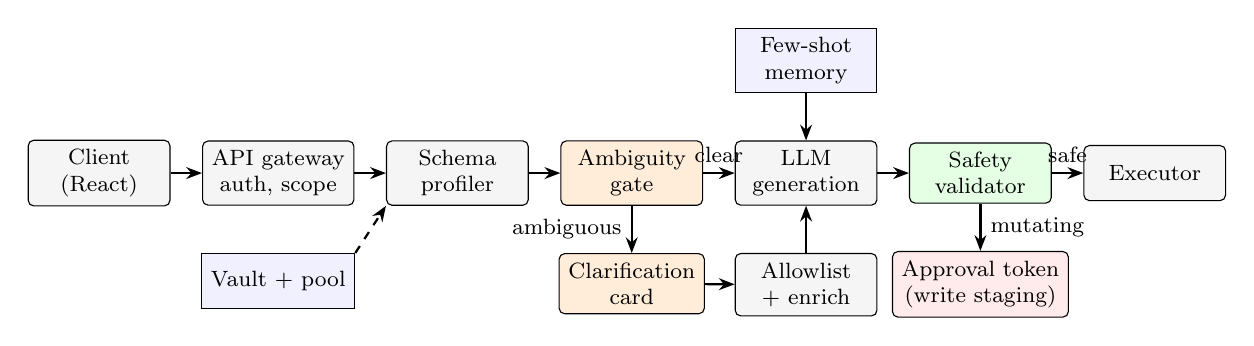
\begin{tikzpicture}[font=\footnotesize,
  box/.style={draw, rounded corners=2pt, minimum height=7mm, minimum width=18mm, align=center, fill=gray!8},
  store/.style={draw, minimum height=7mm, minimum width=18mm, align=center, fill=blue!6},
  arr/.style={-{Stealth[length=2mm]}, thick}, node distance=6mm and 4mm]
\node[box] (client) {Client\\(React)};
\node[box, right=of client] (api) {API gateway\\auth, scope};
\node[box, right=of api] (prof) {Schema\\profiler};
\node[box, right=of prof, fill=orange!15] (gate) {Ambiguity\\gate};
\node[box, right=of gate] (llm) {LLM\\generation};
\node[box, right=of llm, fill=green!10] (val) {Safety\\validator};
\node[box, right=of val] (exec) {Executor};
\node[box, below=of gate, fill=orange!15] (card) {Clarification\\card};
\node[box, below=of llm] (enr) {Allowlist\\+ enrich};
\node[store, below=of api] (vault) {Vault + pool};
\node[store, above=of llm] (mem) {Few-shot\\memory};
\node[box, below=of val, fill=red!8] (hitl) {Approval token\\(write staging)};
\draw[arr] (client)--(api); \draw[arr] (api)--(prof); \draw[arr] (prof)--(gate);
\draw[arr] (gate)--node[above]{clear}(llm);
\draw[arr] (llm)--(val); \draw[arr] (val)--node[above]{safe}(exec);
\draw[arr] (gate)--node[left]{ambiguous}(card);
\draw[arr] (card)--(enr); \draw[arr] (enr)--(llm);
\draw[arr] (mem)--(llm);
\draw[arr] (val)--node[right]{mutating}(hitl);
\draw[arr, dashed] (vault.north east)--(prof.south west);
\end{tikzpicture}
\caption{AMB-MQL request flow. The vault and pool supply database handles to the profiler and executor (dashed).}
\label{fig:arch}
\end{figure*}

\subsection{Schema Profiling and Scope}
For each in-scope collection the profiler draws $N{=}5$ documents with \texttt{\$sample}, records field names, BSON types and one sample value, flattens sub-documents into dot paths (depth at most three), and exposes array-of-object sub-fields as \texttt{field[].sub}. A field present in a fraction $p$ of documents is missed with probability $(1-p)^5$ (about $0.77$ for $p{=}0.05$). A user-chosen collection scope bounds both the schema shown to the model and the validator's permitted collections.

\subsection{Generation}
The prompt contains the current date, the schema string, up to three retrieved question--pipeline examples and aggregation rules (e.g., unwind arrays before grouping). Examples are stored per tenant and retrieved by Atlas Search text query with a regular-expression fallback. A new example is stored after any execution that returns a non-empty result; no further verification is applied (Section~\ref{sec:limitations}).

\subsection{Interpretation-Compliance Verification}
After a clarification, a verifier runs between generation and safety validation and checks that the pipeline implements the chosen metric and sort direction rather than merely mentioning the field: (i)~a \texttt{\$sort} on the target field in the requested direction ($-1$ for ``top''/``highest'', $+1$ for ``lowest''); (ii)~for metrics inside arrays (e.g., \texttt{items[].quantity}), an \texttt{\$unwind} before a \texttt{\$group} using \texttt{\$sum}, \texttt{\$avg}, \texttt{\$max} or \texttt{\$min}; (iii)~resolution of aliases through \texttt{\$addFields} and \texttt{\$project} for computed metrics. It was added after the 100-query run and is active only in Section~\ref{sec:fair}.

\subsection{Validation, Execution, and Write Staging}
Every pipeline passes a recursive key-scan validator that (i)~rejects \texttt{\$function}, \texttt{\$accumulator} and \texttt{\$where} at any depth, (ii)~caps pipelines at 20 stages, (iii)~requires every top-level stage, and every stage nested in \texttt{\$facet}, \texttt{\$lookup.pipeline} and \texttt{\$unionWith.pipeline}, to belong to an 18-stage analytical allowlist (e.g., \texttt{\$match}, \texttt{\$group}, \texttt{\$sort}, \texttt{\$lookup}, \texttt{\$facet}), (iv)~resolves collections referenced by \texttt{\$lookup}, \texttt{\$unionWith}, \texttt{\$graphLookup} and \texttt{\$facet}, including document-form \texttt{from} specifications, and rejects those outside the scope or in the \texttt{admin}, \texttt{config} and \texttt{local} namespaces, and (v)~appends \texttt{\$limit: 1000} when no limit is present.

Pipelines containing \texttt{\$out} or \texttt{\$merge} are not executed directly. They are staged behind an HS256-signed JWT~\cite{jwt2015rfc} valid for ten minutes that binds the pipeline, collection, scope and session, carries a unique identifier consumed once through a unique index, and is re-validated on submission. The token is returned to the requesting session, so it provides confirmation rather than separation of duties. \texttt{\$set} and \texttt{\$unset} only reshape the stream and are allowed.

\subsection{Multi-Tenant Infrastructure}
Connection strings are encrypted with AES-256-CBC~\cite{nist80038a} under a fresh 16-byte IV; the key is read from the environment and the service refuses to start without it. A connection is identified by the SHA-256 digest of its URI. Sessions use an httpOnly cookie holding a seven-day JWT, requests are rate-limited per IP, and database handles are pooled per connection (at most 50 clients, five-minute idle timeout, LRU eviction, ping before reuse). CBC has no integrity tag and the digest is unsalted (Section~\ref{sec:limitations}).

\section{Deterministic Ambiguity Gating}
\label{sec:gate}

\begin{algorithm}[t]
\caption{Deterministic Schema-Grounded Ambiguity Gate}
\label{alg:gate}
\begin{algorithmic}[1]
\Require Natural language query $q$, active collection scope $\mathcal{S}$, sampled schemas $\mathcal{M}$
\Ensure Decision $d \in \{\textsc{Clear}, \textsc{Ask}\}$, candidates $\mathcal{C}$
\State $\mathcal{T}_{\text{vague}} \gets \{\text{``top'', ``best'', ``highest'', ``lowest'', ``most'', ``worst'', \dots}\}$
\State $M_{\text{matched}} \gets \{ t \in \mathcal{T}_{\text{vague}} \mid t \text{ matches word boundary in } q \}$
\If{$M_{\text{matched}} = \emptyset$}
    \State \Return $(\textsc{Clear}, \emptyset)$
\EndIf
\State $\mathcal{F}_{\text{num}} \gets \bigcup_{c \in \mathcal{S}} \textsc{ExtractNumericMetricCandidates}(\mathcal{M}[c])$
\If{$|\mathcal{F}_{\text{num}}| < 2$}
    \State \Return $(\textsc{Clear}, \emptyset)$
\EndIf
\State $\mathcal{B}_{\text{bound}} \gets \textsc{DetectHeuristicFieldBinding}(q, \mathcal{F}_{\text{num}})$
\If{$\mathcal{B}_{\text{bound}} \neq \emptyset \lor \textsc{IdiomaticCollocation}(q, M_{\text{matched}})$}
    \State \Return $(\textsc{Clear}, \emptyset)$ \Comment{Explicitly bound}
\EndIf
\State $\mathcal{C} \gets \textsc{TopCandidates}(\mathcal{F}_{\text{num}}, \text{limit}=4)$
\State \Return $(\textsc{Ask}, \mathcal{C})$
\end{algorithmic}
\end{algorithm}

\subsection{Trigger Terms, Binding and Clarification Cards}
The 15 trigger terms are: top, best, highest, lowest, most, worst, greatest, least, cheapest, priciest, maximum, minimum, max, min, largest. On a word-boundary match, the gate extracts numeric candidates $\mathcal{F}_{\text{num}}$ from the profiled schemas by inspecting the trailing segment of each dot path, accepting numeric BSON types and filtering identifier-like (\texttt{\_id}, \texttt{customerId}) and year-like fields. If $|\mathcal{F}_{\text{num}}| \ge 2$ and no field is bound, the gate emits a card with up to four candidates, truncated alphabetically or by sample order, plus an ``Other'' option. A field is bound when its leaf name or a schema synonym lies within $\delta{=}3$ tokens of the trigger term (with bidirectional metric-verb grounding) or an explicit phrase such as ``by price'' appears. A collocation guard suppresses idiomatic non-metric uses (e.g., ``at least one''). Without these two additions (the \emph{baseline gate}), UCR is \gateBaseUCR{}.

\subsection{Execution Latency}
The gate runs in-process on compiled regular expressions and cached schemas. Mean latency was \gateLatencyMean{} (median \gateLatencyPFifty{}, p99 \gateLatencyPNineNine{}; \gateBaseLatencyMean{} for the baseline gate), against a median end-to-end time of 1.2--1.4\,s.

\section{Clarification Handling}
\label{sec:safety}
A bypass suppresses re-prompting; ``Other'' requests a free-text metric; any other selection must belong to both the offered set and the profiled schema, otherwise HTTP 422 is returned. A valid selection is appended to the prompt as ``Disambiguated target metric: $\langle\text{field}\rangle$'' and checked by the compliance verifier.

\section{Experimental Setup}
\label{sec:setup}

\subsection{Benchmark Construction and Datasets}
The benchmark has \numTotalQueries{} execution-verified queries over three Atlas sample datasets: \texttt{sample\_supplies} (sales with nested line items), \texttt{sample\_analytics} (accounts and transactions) and \texttt{sample\_mflix} (movies, comments, awards). Queries fall into five categories: \texttt{AMB\_LEX} (a trigger term and $\ge 2$ numeric candidates), \texttt{AMB\_PARA} (ambiguity by paraphrase, no trigger term), \texttt{CLR\_FIELD} (the metric is named despite a dense schema), \texttt{CLR\_BOUND} (explicit bounds or limits) and \texttt{CLR\_PLAIN} (projection, counting, exact match). The finalized benchmark contains \numAmbiguousQueries{} ambiguous and \numClearQueries{} clear queries. In 31 queries the scope offers fewer than two numeric candidates, so the gate returns clear by design.

The gate is scored on \gateScoredN{} queries ($N_{\text{amb}} = 69$, $N_{\text{clear}} = 249$). Twelve queries with conversational temporal references (e.g., \emph{``Show the purchases from the relevant period''}) are marked \texttt{OOS\_UNSCORED} and excluded, because the gate targets metric ambiguity rather than temporal resolution; Table~\ref{tab:gate_metrics} reports recall if they are counted as misses. The 69 scored ambiguous queries are 38 \texttt{AMB\_LEX}, 26 \texttt{AMB\_PARA} and 5 aggregation-grain queries (\texttt{CLR\_AGG}, e.g., \emph{``Count transactions for each customer age group''}) that annotators judged ambiguous because the bucket interval is unspecified.

\subsection{Human Annotation and Inter-Annotator Agreement}
Annotator~A (intermediate MongoDB experience) labelled all \numTotalQueries{} queries; annotator~B (beginner) independently labelled \numDoubleLabelAll{} of them (29\%) under a shared guide, without code inspection, so the remaining 235 labels rest on one annotator. Agreement is computed on the binary ambiguous/clear label. Across all \numDoubleLabelAll{} double-labelled queries, observed agreement is \observedAgreementAll{} ($93/95$), $\kappa = \cohenKappaAll{}$, $\text{PABAK} = \pabakAll{}$. The two disagreements fall among four incidentally annotated rows (\texttt{mflix-0300}, \texttt{mflix-0314}) outside the designated stratified sample ($\kappa = \cohenKappaStratified{}$ on \numDoubleLabelStratified{} queries). Because \texttt{AMB\_LEX} is defined by trigger vocabulary, high agreement on it reflects rule application rather than independent judgement; the lexical recall below is likewise definitional.

\subsection{Evaluation Configurations and LLM Infrastructure}
For end-to-end evaluation, we evaluate a representative stratified subset of \eTwoETotalQueries{} queries drawn as 55 queries designed as ambiguous (35 \texttt{AMB\_LEX}, 20 \texttt{AMB\_PARA}) and 45 gold-verified clear queries (15 each \texttt{CLR\_FIELD}, \texttt{CLR\_BOUND}, \texttt{CLR\_PLAIN}). We score against the annotators' labels: \eTwoEAmbiguousQueries{} are ambiguous (22 \texttt{AMB\_LEX}, 16 \texttt{AMB\_PARA}) and \eTwoEClearQueries{} are clear, because annotators judged 17 of the 55 designed-ambiguous queries clear (13 \texttt{AMB\_LEX}, 4 \texttt{AMB\_PARA}). We evaluate three configurations:
\begin{itemize}
    \item \textbf{C0a (Zero-ARL Baseline):} Standard single-pass generation with clarification disabled (\texttt{disableClarificationMode: true}), measuring raw baseline silent assumption susceptibility.
    \item \textbf{C0b (LLM-Only Baseline):} Conversational generation where the model autonomously chooses between synthesizing a query or requesting clarification (\texttt{needsClarification: true}).
    \item \textbf{C2 (AMB-MQL):} In-process deterministic gate pre-filter $\to$ allowlist-validated clarification card $\to$ single-call generation $\to$ compliance check (fair comparison only) $\to$ safety validation.
\end{itemize}
All configurations use the open-weights model \texttt{openai/gpt-oss-120b} hosted on Groq. In the 100-query run, C2 used the baseline gate and no compliance verifier; the extended gate is evaluated on the 318-query gate benchmark, on the clear-query interruption count, and in the fair comparison below.

A second, \emph{fair} comparison uses a uniform simulator and a one-turn budget for C0b and C2, so gate cards and model questions are answered identically: each ambiguous query has a hidden intended metric; the simulator picks it from offered options (or ``Other'' with the metric text if truncated), answers open questions with the intended interpretation (no reference MQL), and bypasses on clear queries. Unresolved queries after one turn count as failures. It uses a balanced sample of $N{=}25$ (10 ambiguous, 15 clear).

\section{Empirical Results}
\label{sec:results}

\subsection{Deterministic Ambiguity Gate Evaluation}
Table~\ref{tab:gate_metrics} reports the baseline gate and the extended gate (proximity binding and collocation guard) on the \numTotalQueries{}-query test split ($N_{\text{scored}} = \gateScoredN{}$, evaluating the 69 candidate-evaluated ambiguous and 249 clear queries, excluding 12 \texttt{OOS\_UNSCORED} temporal reference queries).

\begin{table*}[t]
\centering
\caption{Deterministic Ambiguity Gate Evaluation on Test Split ($N = 330$, $N_{\text{scored}} = 318$).}
\label{tab:gate_metrics}
\begin{tabular}{lcccc}
\toprule
\textbf{Metric} & \textbf{Baseline gate} & \textbf{Proximity + colloc.\ guard} & \textbf{$\Delta$} & \textbf{$n$ / Notes} \\
\midrule
Lexical recall (\texttt{AMB\_LEX}) & 100.0\%~{\scriptsize[90.8, 100.0]} & 100.0\%~{\scriptsize[90.8, 100.0]} & 0 & 38; definitional$^{\dagger}$ \\
Paraphrase recall (\texttt{AMB\_PARA}) & 0.0\%~{\scriptsize[0.0, 12.9]} & 0.0\%~{\scriptsize[0.0, 12.9]} & 0 & 26; LLM handles \\
Aggregation recall (\texttt{CLR\_AGG}) & 0.0\%~{\scriptsize[0.0, 43.4]} & 0.0\%~{\scriptsize[0.0, 43.4]} & 0 & 5; LLM handles \\
Overall recall & 55.1\%~{\scriptsize[43.4, 66.2]} & 55.1\%~{\scriptsize[43.4, 66.2]} & 0 & 69 \\
\midrule
Precision / F1 & 25.3\%~{\scriptsize[19.0, 32.8]} / 34.7\% & \textbf{52.1\%}~{\scriptsize[40.8, 63.1]} / 53.5\% & +26.8\,pp & $\text{TP}/(\text{TP}{+}\text{FP})$ \\
Specificity & 55.0\%~{\scriptsize[48.8, 61.1]} & \textbf{85.9\%}~{\scriptsize[81.1, 89.7]} & +30.9\,pp & 249 clear \\
UCR & 45.0\%~{\scriptsize[38.9, 51.2]} & \textbf{14.1\%}~{\scriptsize[10.3, 18.9]} & $-$30.9\,pp & $1-\text{Specificity}$ \\
\midrule
\textbf{Confusion} & \multicolumn{2}{c}{TP 38, FP $112{\to}35$, TN $137{\to}214$, FN 31} & \multicolumn{2}{c}{$-77$ FP ($-68.8\%$)} \\
\midrule
\multicolumn{5}{l}{\textbf{False-positive root causes (baseline $n{=}112$):}} \\
\quad Bound misses (\texttt{CLR\_BOUND}) & 42 (37.5\%) & 0 & $-42$ & resolved by proximity ($\delta{=}3$) \\
\quad Schema density (\texttt{CLR\_FIELD}) & 33 (29.5\%) & 0 & $-33$ & resolved by leaf/synonym binding \\
\quad Collocations (\texttt{CLR\_PLAIN}) & 2 (1.8\%) & 0 & $-2$ & resolved by collocation guard \\
\quad Field named (\texttt{AMB\_LEX}, annotated clear) & 35 (31.3\%) & 35 & 0 & residual: human vs.\ literal schema \\
\midrule
Mean latency (p50) & 14.61\,$\mu$s (12.9) & 129.07\,$\mu$s (105.8) & +114.5\,$\mu$s & in-process \\
\bottomrule
\end{tabular}
\\[2pt]
\footnotesize{$^{\dagger}$Lexical-term categories report recall as definitional: by construction, the gate triggers whenever $\ge 2$ numeric candidates match an active vagueness token. The 69 ambiguous queries comprise 38 lexical candidates, 26 paraphrased queries, and 5 unbucketed aggregation queries. Ground truth is the annotated label and requires at least two numeric candidates in scope; two annotated-ambiguous queries with fewer are scored clear. Of 73 queries generated as \texttt{AMB\_LEX}, 38 were annotated ambiguous. Twelve temporal queries (all annotated ambiguous) are \texttt{OOS\_UNSCORED}; the gate asked on one, so counting them gives recall $39/81 = 48.1\%$.}
\end{table*}

Recall is \gateRecallLexical{} on \texttt{AMB\_LEX} (definitional) and 0.0\% on paraphrases and aggregation-grain queries; overall recall is \gateRecallOverall{}. The baseline gate had specificity \gateBaseSpecificity{}, UCR \gateBaseUCR{} and precision \gateBasePrecision{}. Proximity binding and the collocation guard removed 77 of 112 false positives: specificity \gateSpecificity{}, UCR \gateUCR{}, precision \gatePrecision{}, recall unchanged. The 35 residual false positives are named-field queries that annotators judged settled while the schema still offers several candidates.

\subsection{End-to-End Generation Comparison}
Table~\ref{tab:e2e_comparison} compares C0a, C0b and C2 on a stratified subset of $N = \eTwoETotalQueries{}$ queries ($n = \eTwoEAmbiguousQueries{}$ ambiguous, $n = \eTwoEClearQueries{}$ clear). Silent assumptions are counted when a pipeline is returned without any gate or LLM clarification.

\begin{figure}[t]
\centering
\definecolor{c0ablue}{RGB}{37, 137, 252}
\definecolor{c0borange}{RGB}{234, 110, 41}
\definecolor{c2teal}{RGB}{0, 168, 133}
\begin{tikzpicture}
\begin{axis}[
  ybar=1pt, bar width=6.5pt, width=\columnwidth, height=4.6cm,
  ymin=0, ymax=118, ytick={0, 25, 50, 75, 100},
  ylabel={Silent assumption rate (\%)},
  symbolic x coords={All (38), LEX (22), PARA (16)},
  xtick=data, x tick label style={font=\footnotesize}, nodes near coords,
  nodes near coords style={font=\tiny, /pgf/number format/fixed, /pgf/number format/precision=1},
  legend style={at={(0.5, 1.04)}, anchor=south, legend columns=-1, font=\footnotesize, draw=none,
    /tikz/every even column/.append style={column sep=0.3cm}},
  enlarge x limits=0.25, ymajorgrids=true, grid style={dashed, gray!30}
]
\addplot[fill=c0ablue, draw=c0ablue!80!black] coordinates {(All (38), 100) (LEX (22), 100) (PARA (16), 100)};
\addplot[fill=c0borange, draw=c0borange!80!black] coordinates {(All (38), 65.8) (LEX (22), 81.8) (PARA (16), 43.8)};
\addplot[fill=c2teal, draw=c2teal!80!black] coordinates {(All (38), 18.4) (LEX (22), 0) (PARA (16), 43.8)};
\legend{C0a: Zero-ARL, C0b: LLM-only, C2: AMB-MQL}
\end{axis}
\end{tikzpicture}
\caption{Silent assumption rate on annotator-ambiguous queries (lower is better); LEX = \texttt{AMB\_LEX}, PARA = \texttt{AMB\_PARA}; $n$ in parentheses.}
\label{fig:silent}
\end{figure}

\begin{table*}[t]
\centering
\caption{End-to-End Generation Comparison across Baselines and AMB-MQL on \texttt{openai/gpt-oss-120b} ($N = 100$).}
\label{tab:e2e_comparison}
\resizebox{\textwidth}{!}{%
\begin{tabular}{lcccc}
\toprule
\textbf{Evaluation Metric \& Subset Scope} & \textbf{C0a: Zero-ARL} & \textbf{C0b: LLM-Only} & \textbf{C2: AMB-MQL} & \textbf{Paired Difference [95\% CI]} \\
\midrule
\multicolumn{5}{l}{\textbf{1. Silent Assumption Rate (Lower is Better, Denominator: Ambiguous Queries)}} \\
\quad All Ambiguous Queries ($n = 38$) & \eTwoECZeroASilentAmb{}~{\scriptsize[90.8\%, 100.0\%]} & \eTwoECZeroBSilentAmb{}~{\scriptsize[49.9\%, 78.8\%]} & \textbf{\eTwoECTwoSilentAmb{}}~{\scriptsize[9.2\%, 33.4\%]} & $\Delta = \eTwoESilentAmbDelta{}$~{\scriptsize[31.6, 63.2]} ($p = \eTwoESilentAmbMcNemarP{}$)$^{\dagger}$ \\
\quad \texttt{AMB\_LEX} ($n = 22$) & 100.0\%~{\scriptsize[85.1\%, 100.0\%]} & 81.8\%~{\scriptsize[61.5\%, 92.7\%]} & \textbf{0.0\%}~{\scriptsize[0.0\%, 14.9\%]} & $-81.8\,\text{pp}$ vs.\ C0b \\
\quad \texttt{AMB\_PARA} ($n = 16$) & 100.0\%~{\scriptsize[80.6\%, 100.0\%]} & 43.8\%~{\scriptsize[23.1\%, 66.8\%]} & 43.8\%~{\scriptsize[23.1\%, 66.8\%]} & Gate silent; LLM asks on 56\% \\
\midrule
\multicolumn{5}{l}{\textbf{2. Target Verification Accuracy (Higher is Better)}} \\
\quad Intended Metric Match (\texttt{AMB\_LEX}, $n = 22$)$^{\ddagger}$ & 63.6\%~{\scriptsize[43.0\%, 80.3\%]} & 50.0\%~{\scriptsize[30.7\%, 69.3\%]} & \textbf{100.0\%}~{\scriptsize[85.1\%, 100.0\%]} & Grounded candidate selection \\
\quad Intended Metric Match (\texttt{AMB\_PARA}, $n = 16$)$^{\ddagger}$ & 37.5\%~{\scriptsize[18.5\%, 61.4\%]} & 18.8\%~{\scriptsize[6.6\%, 43.0\%]} & 18.8\%~{\scriptsize[6.6\%, 43.0\%]} & Parity (LLM asks unanswered) \\
\quad Gold Result Match, pre-audit raw ($n = 45$)$^{\ddagger}$ & 80.0\%~{\scriptsize[66.2\%, 89.1\%]} & 80.0\%~{\scriptsize[66.2\%, 89.1\%]} & 77.8\%~{\scriptsize[63.7\%, 87.5\%]} & 36/45, 36/45, 35/45 (legacy comparator) \\
\quad Gold Result Match, post-audit reconciled ($n = 45$)$^{\mathsection}$ & 100.0\%~{\scriptsize[92.1\%, 100.0\%]} & 100.0\%~{\scriptsize[92.1\%, 100.0\%]} & 100.0\%~{\scriptsize[92.1\%, 100.0\%]} & Derived: $36{+}9$, $36{+}9$, $35{+}10$ of 45 \\
\midrule
\multicolumn{5}{l}{\textbf{3. Valid Pipeline Rate}} \\
\quad Clear queries ($n = 62$) & 100.0\%~{\scriptsize[94.2\%, 100.0\%]} & 90.3\%~{\scriptsize[80.5\%, 95.5\%]} & 95.2\%~{\scriptsize[86.7\%, 98.3\%]} & Unanswered LLM asks \\
\quad Gold-verified clear ($n = 45$) & 100.0\%~{\scriptsize[92.1\%, 100.0\%]} & 100.0\%~{\scriptsize[92.1\%, 100.0\%]} & 100.0\%~{\scriptsize[92.1\%, 100.0\%]} & Executes; says nothing on correctness \\
\quad Overall ($n = 100$) & 100.0\%~{\scriptsize[96.3\%, 100.0\%]} & 81.0\%~{\scriptsize[72.2\%, 87.5\%]} & \textbf{88.0\%}~{\scriptsize[80.2\%, 93.0\%]} & $+7.0\,\text{pp}$ (C0b clarification pause) \\
\midrule
\multicolumn{5}{l}{\textbf{4. Clarification Rate \& Interaction Overhead}} \\
\quad Gate-Initiated Clarifications, baseline gate ($n = 100$)$^{\mathparagraph}$ & 0.0\% & 0.0\% & \textbf{59.0\%} & 35 ambiguous + 24 clear \\
\quad LLM-Initiated Clarifications ($n = 100$) & 0.0\% & 19.0\% & \textbf{12.0\%} & Paraphrase LLM fallback prompts \\
\quad Unnecessary interruption, baseline gate (clear, $n = 62$)$^{\mathparagraph}$ & 0.0\% & 9.7\%~{\scriptsize[4.5\%, 19.5\%]} & 64.5\%~{\scriptsize[52.1\%, 75.3\%]} & 40/62; 24/45 gold-verified (53.3\%) \\
\quad Unnecessary interruption, extended gate (clear, $n = 62$) & 0.0\% & 9.7\%~{\scriptsize[4.5\%, 19.5\%]} & \textbf{41.9\%}~{\scriptsize[30.5\%, 54.3\%]} & 26/62; $-22.6$\,pp vs.\ baseline gate \\
\midrule
\multicolumn{5}{l}{\textbf{5. Cost}} \\
\quad Mean tokens / query & 1911.8 & 1883.3 & 1895.2 & Gate adds no tokens \\
\quad Median / mean latency (s) & 1.40 / 18.80 & 1.38 / 19.28 & 1.23 / 19.82 & Means dominated by ${\approx}58$\,s outliers (31--33 per config) \\
\bottomrule
\end{tabular}%
}
\\[2pt]
\footnotesize{$^{\dagger}$Paired statistical difference evaluated on matched $n = 38$ annotator-ambiguous queries via exact two-sided McNemar test ($b = 18$, $c = 0$) and a paired bootstrap CI. Over all 55 designed-ambiguous queries, counting a silent assumption as a pipeline returned without any clarification, the rates are 100.0\%, 65.5\% and 14.5\% ($\Delta = -50.9\,\text{pp}$, bootstrap CI [38.2, 63.6]; $b = 28$, $c = 0$, $p = 7.45\times 10^{-9}$).}\\
\footnotesize{$^{\ddagger}$Formula: Multiset equality evaluated on 4-decimal rounded, Decimal128-normalized documents. For ambiguous queries, match evaluates recovery of the ground-truth candidate interpretation. Clear queries are evaluated on execution equivalence against reference gold pipeline. The raw row's 9 shared misses (all \texttt{CLR\_PLAIN}, \texttt{sample\_supplies}) and the one C2-only miss (\texttt{supplies-0017}) were comparator artifacts: the legacy harness checked a dummy \texttt{price} token on non-price filters.}\\
\footnotesize{$^{\mathsection}$Derived, not re-measured: the 10 audited queries re-scored under the corrected semantic predicate and added back.}\\
\footnotesize{$^{\mathparagraph}$Measured with the baseline gate, before proximity binding ($\delta{=}3$) and the collocation guard. Gate-initiated clarifications under the extended gate were not re-reported.}
\end{table*}

C0a answers all ambiguous queries silently (38/38); C0b lowers this to \eTwoECZeroBSilentAmb{} (25/38); C2 to \eTwoECTwoSilentAmb{} (7/38), a paired reduction of \eTwoESilentAmbDelta{} (McNemar $p = \eTwoESilentAmbMcNemarP{}$). As Fig.~\ref{fig:silent} shows, the gain is entirely on \texttt{AMB\_LEX}; on \texttt{AMB\_PARA} the gate is silent and C2 equals C0b. Subgroup intervals are wide.

The price is interaction: the baseline gate interrupted 40 of 62 clear queries (64.5\%), the extended gate 26 (41.9\%), against 6 for C0b. The oracle's bypass lets all 45 gold-verified queries execute; a real user could pick a wrong option. Unanswered LLM questions lower the valid-pipeline rates of C0b and C2. The legacy comparator's 10 artifacts (Section~\ref{sec:audit}) explain the raw-to-reconciled gold match.

\subsection{Fair Comparison under a Uniform Simulator}
\label{sec:fair}
Table~\ref{tab:fair} uses a uniform simulator and one-turn budget ($N{=}25$). C2 lowers silent assumptions from 60.0\% to 20.0\% (0.0\% on lexical cues) at equal correctness (80.0\%) and 0/15 unnecessary clarifications; the verifier was not ablated, and C2 asks more (0.32 vs.\ 0.16 turns). The $n{=}10$ ambiguous subset is small.

\begin{table}[t]
\centering\footnotesize
\caption{Uniform simulator, one-turn budget ($N{=}25$).}
\label{tab:fair}
\begin{tabular}{lccc}
\toprule
\textbf{Metric} & \textbf{C0a} & \textbf{C0b} & \textbf{C2} \\
\midrule
Final result correctness & 84.0\% & 80.0\% & 80.0\% \\
Silent assumption ($n{=}10$) & 100.0\% & 60.0\% & \textbf{20.0\%} \\
Unnecessary clarification ($n{=}15$) & 0.0\% & 0.0\% & 0.0\% \\
Mean clarification turns & 0.00 & 0.16 & 0.32 \\
Unresolved requests & 0.0\% & 16.0\% & 12.0\% \\
Model calls / query & 1.00 & 1.16 & 1.12 \\
Mean prompt tokens / query & 1,878 & 1,863 & 1,867 \\
\bottomrule
\end{tabular}
\end{table}

\subsection{Independent Query Set}
Twenty-five queries written without knowledge of the trigger terms (five per category) produced no false positives on clear queries, routed all five absent-schema requests to ``Other'', and reached 20.0\% recall on non-trigger ambiguity.

\subsection{Audited Mismatches and Ordering Semantics}
\label{sec:audit}
Ten mismatches (\texttt{supplies-0004}--\texttt{0017}) were comparator artifacts: the legacy harness checked a placeholder \texttt{price} token on non-price filters. Under the corrected predicate all ten are correct in C0a, C0b and C2. The comparator uses multiset equality for unranked queries and strict list equality for ranking queries.

\subsection{Safety Guard and Adversarial Resistance}
The validator was tested on 259 author-written pipelines and five token-replay checks. All 135 adversarial pipelines were rejected (100.0\%, 95\% CI [97.2\%, 100.0\%]), covering scope violations, mutating stages, code execution, nested administrative sub-pipelines, foreign namespaces and oversized pipelines. All 124 benign analytical pipelines were allowed (CI [97.0\%, 100.0\%]). All five replay checks were blocked: session mismatch (403), JTI double spend (409), signature tampering (401), hard-deny revalidation tamper (422) and expired token (401).
Because the suite was written by the authors, it demonstrates the allowlist's behaviour on known vectors rather than coverage of unknown ones.

\section{Related Work}
\label{sec:related}

\subsection{NLIDBs and Text-to-NoSQL}
Relational NLIDBs~\cite{quamar2022nli,ozcan2020nli} are driven by Spider~\cite{spider2018} and BIRD~\cite{bird2023}, with decomposed and in-context methods such as DIN-SQL~\cite{dinsql2023} and DAIL-SQL~\cite{dailsql2023}. Hossen et al.~\cite{hossen2023bert} and Blank et al.~\cite{blank2019nosql} predict elementary CRUD operations with neural encoders, without aggregation support or ambiguity handling. DocSpider~\cite{docspider2025} and SM3-Text-to-Query~\cite{sm3text2024} extend evaluation to cross-domain and multi-model document querying, again with one intended answer per request. TEND and MultiTEND~\cite{tend2025benchmark,multitend2025} report below 36\% execution accuracy without instance-level grounding; their tasks have a single intended answer and no pre-generation ambiguity detection, and SAG's 400-document grounding is richer than our five-document profile.

\subsection{Ambiguity and Clarification}
For SQL, AmbiQT~\cite{bhaskar2023ambiqt} and AMBROSIA~\cite{saparina2024ambrosia} benchmark questions with several valid queries, DTE~\cite{wang2023dte} labels ambiguous tokens, and Sphinteract~\cite{zhao2025sphinteract} asks multiple-choice questions to resolve column ambiguity and weighs accuracy against interaction rounds. We are not aware of an equivalent for MongoDB. Ours is a zero-LLM-call, schema-grounded gate for one ambiguity type (metric choice) in aggregation pipelines.

\section{Threats to Validity and System Limitations}
\label{sec:limitations}

\begin{enumerate}
    \item \textbf{Lexical gate.} The 15-term dictionary gives \gateRecallLexical{} recall on \texttt{AMB\_LEX} by construction and \gateRecallParaphrase{} on paraphrases and aggregation-grain ambiguity; those depend on LLM-initiated clarification. On 25 independently written queries, recall on non-trigger ambiguity was 20.0\% (1/5). The gate handles metric ambiguity only, not array grain, join direction or stage order.
    \item \textbf{Four-candidate truncation.} In dense collections the card can omit the intended field, forcing ``Other''.
    \item \textbf{Memory and verifier.} Stored examples are not checked against the chosen metric; the verifier covers only direct-field ranking, single-hop grouping and aliases. Evaluation is limited to \numTotalQueries{} queries, three datasets, one model, student annotators, and an asymmetric harness (Section~\ref{sec:fair}).
    \item \textbf{Sampling.} Five sampled documents can miss sparse numeric fields, changing $\mathcal{F}_{\text{num}}$ and the card.
    \item \textbf{Safety evaluation.} The adversarial suite is author-written and does not replace fuzzing.
    \item \textbf{Credentials.} AES-256-CBC lacks an integrity tag and URI digests are unsalted; we plan AES-256-GCM and salted HMAC.
\end{enumerate}

\section{Conclusion}
\label{sec:conclusion}

We presented AMB-MQL, which places a deterministic, schema-grounded gate (\gateLatencyMean{} mean, no tokens) before a single model call, followed by compliance verification, allowlist validation and signed write staging. The gate removes silent assumptions on lexically cued ambiguity (\eTwoECTwoSilentLex{} vs.\ \eTwoECZeroASilentLex{} in C0a) and lowers overall silent assumptions by \eTwoESilentAmbDelta{} ($p = \eTwoESilentAmbMcNemarP{}$), but does not help on paraphrased ambiguity, and its \gateUCR{} unnecessary-clarification rate remains a real cost. Answering LLM-initiated questions in the full 100-query run is the next step.

\bibliographystyle{IEEEtran}
\bibliography{\jobname}
\end{document}